\chapter{Results}
\label{res}
The whole microprocessor was synthesized inside ``Synopsys Design Compiler'' thanks to the ``./synthesis/DLX\_synth.scr'' dedicated script (together with the provided \texttt{.synopsys\_dc.setup} configuration file). There, an unconstrained cycle is executed first, then synchronous, combinational and low-power constraints are applied in order to perform a subsequent optimization process.

The specific values that are required to perform this step were found by hand, after a streak of \emph{trial and error} synthesis runs, and the ensuing outcomes were automatically generated in ``./synthesis/report/''. The output netlists resulting from this process were finally used as input for the physical design step, that was ultimately carried out inside ``Cadence Innovus Implementation System''.

Note that Memories were excluded from the above operations, as indicated by the guidelines of this project.

\section{Area}
The following results were extracted after the optimization phase of the top-level entity:
\verbatiminput{chapters/files/1-DLX_area_opt.rpt}

\section{Timing}
After applying the following clock period:
\verbatiminput{chapters/files/1-DLX_clock_opt.rpt}
the most critical path was found to be the one going from an internal flip-flop of the \nameref{control-unit} (more specifically, bit number 12 of the control word dedicated to managing the Execute stage) till the flip-flop that manages the Zero flag inside the \nameref{cpsr}:
\verbatiminput{chapters/files/1-DLX_timing_opt.rpt}

\section{Power}
After the low-power synthesis step, the imposed constraint was finally conformed to, and the main contributions to this physical quantity were found to be as follows:
\verbatiminput{chapters/files/1-DLX_power_opt.rpt}

\section{Physical Design}
The post-synthesis Verilog netlist was used as input for the entire physical design process, which would in turn generate, among many other valuable resources, the post place and route one. Please note that all files with the ``DLX\_PRO'' title are just the starting point of this step (deriving from the previous one), while all its actual outputs were saved with the ``DLX`` tag only.

All the produced dumps, archives and reports are located inside the ``./physical\_design/'' directory, including all its subfolders for timing information. Many intrinsic characteristics of the final circuit can be found in there, including parasitics, geometry and connectivity characterization.

\begin{figure}[!ht]
\centering
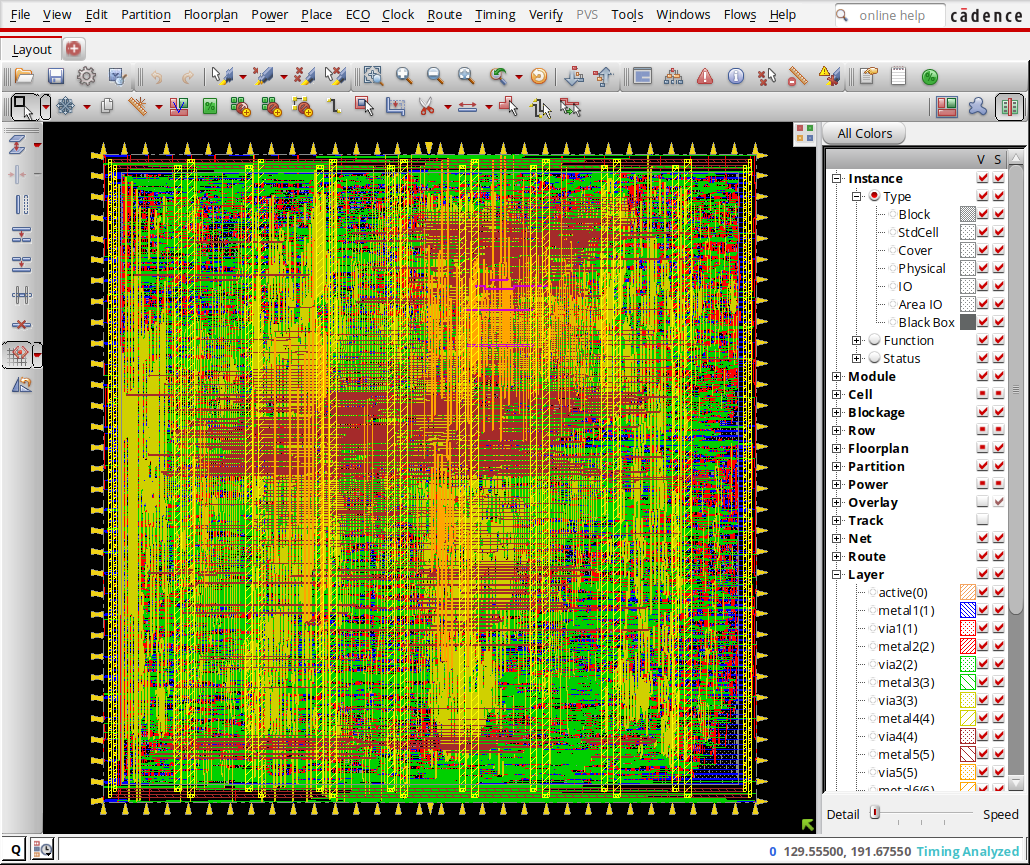
\includegraphics[width=\textwidth]{./chapters/figures/DLX_dump.png} 
\caption{Obtained image dump of the circuit layout.}
\end{figure}